\chapter{Resultados e Discussões}

Neste capítulo são apresentados e discutidos os resultados originados da metodologia proposta para a otimização de manobras de evasão de colisão (CAMO) via simulador em Python, utilizando propagações analíticas e numéricas sob o framework Orekit. A presente análise restringe-se ao período de 19 de fevereiro de 2026 às 12:00:00 UTC até 24 de fevereiro de 2026 às 12:00:00 UTC.

\section{Caracterização dos Satélites de Estudo}

Para a avaliação dos algoritmos propostos, selecionaram-se três satélites de referência, todos operacionais em Órbita Terrestre Baixa (LEO), os quais figuram como alvos primários em potenciais cenários de conjunções: SPACEMOBILE-005 (NORAD ID 61046), KUIPER-00084 (NORAD ID 64830) e KUIPER-00155 (NORAD ID 65774). A seguir, detalham-se as missões e propriedades nominais, além dos elementos orbitais de cada ativo. Ressalta-se que, para fins de simulações da física do propagador ao longo deste trabalho, adotou-se um perfil padrão com massa de $1000,0\text{ kg}$, área de seção transversal de $2,0\text{ m}^2$, coeficiente de arrasto aerodinâmico ($C_D$) avaliado em $2,2$ e coeficiente de refletividade de pressão de radiação solar ($C_R$) ajustado para $1,2$.

\subsection{SPACEMOBILE-005 (Satélite 61046)}

A escolha deste satélite como objeto de estudo principal baseia-se nas grandes dimensões da sua matriz de antenas. Por possuir uma área física significativamente maior do que a média dos satélites comerciais, este veículo apresenta uma chance intrinsecamente elevada de sofrer potenciais colisões espaciais. Essa característica construtiva o consolida como um alvo de análise ideal, visto que sua grande seção transversal aumenta a severidade geométrica natural dos encontros mapeados na \textit{Concern List}, testando rigorosamente a capacidade de busca por soluções de evasão do algoritmo.

Parte da constelação SpaceMobile, este veículo é voltado à prestação de serviços de telecomunicações via conectividade celular direta da órbita LEO. O satélite gravita em trajetória circular, mantendo altitude média de 502 km, com inclinação orbital de $52,98^\circ$. Registrado como SPACEMOBILE-005 (NORAD ID 61046), o ativo estadunidense foi lançado em 12 de setembro de 2024 pelo Polígono de Testes do Leste da Força Aérea (AFETR), a bordo do veículo de lançamento Falcon 9. No que tange às características físicas documentadas de sua estrutura real orbitando a Terra, destaca-se o impressionante valor transversal aferido para a Seção de Radar (RCS), catalogado em exatos $32,59\text{ m}^2$ \citeonline{CELESTRAK_SATCAT}.

\begin{figure}[ht]
    \caption{Imagem do satélite SPACEMOBILE-005.}
    \vspace{3mm}
    \begin{center}
        \includegraphics[width=\mylenfig]{docs/figuras/spacemobile_005.jpeg}  
    \end{center}
    \vspace{4mm}
    \legenda{O satélite SPACEMOBILE-005 em configuração orbital desdobrada, operando com antena faseada na região LEO.}
    \label{fig:sat_61046}
    \FONTE{Adaptada de \citeonline{TOTALTELE2026}.}
\end{figure}

Os parâmetros orbitais clássicos e físicos extraídos da época inicial estão apresentados na Tabela \ref{tab:sat_61046}. Ressalta-se que o termo dissipativo de arrasto é inerentemente modelado pelo parâmetro modificado $B^*$, expresso em inversos de raios terrestres ($ER^{-1}$), em conformidade geométrica com a formulação analítica do propagador SGP4 discutida detalhadamente na Seção \ref{subsec:propagadores} do Capítulo \ref{chap:fundamentacao_teorica}.

\begin{table}[H]
    \centering
    \caption{Elementos Orbitais Clássicos e Físicos - SPACEMOBILE-005 (Satélite 61046)}
    \label{tab:sat_61046}
    \begin{tabular}{lc}
        \toprule
        \textbf{Parâmetro} & \textbf{Valor} \\
        \midrule
        Semieixo Maior ($a$) & $6880,400\text{ km}$ \\
        Excentricidade ($e$) & $0,00124$ \\
        Inclinação ($i$) & $52,98^\circ$ \\
        RAAN ($\Omega$) & $127,27^\circ$ \\
        Argumento do Perigeu ($\omega$) & $128,84^\circ$ \\
        Anomalia média na época ($M$) & $231,36^\circ$ \\
        Movimento Médio ($n$) & $15,21\text{ rev/dia}$ \\
        Período Orbital ($T$) & $94,67\text{ min}$ \\
        BSTAR & $0,42416\times 10^{-3} \text{ ER}^{-1}$ \\
        \bottomrule
    \end{tabular}
\end{table}

\subsection{KUIPER-00084 (Satélite 64830)}

A inclusão de objetos desta matriz operacional estadunidense tem como objetivo testar o algoritmo frente a frotas de satélites em megaconstelações. A seleção destes veículos justifica-se pelo fato de que ativos inseridos em arquiteturas densas recebem altos volumes de alertas de conjunção concorrentes dentro de um curto espaço de tempo. Este cenário exige dos centros de controle soluções automatizadas e rápidas para o planejamento de manobras de evasão, validando a aplicação e a arquitetura do \textit{Smart Sieve} proposto neste trabalho.

Pertencente à rede de constelação do Projeto Kuiper (operada pela Amazon), este veículo atua na veiculação de dados visando prover internet de baixa latência em nível global. O objeto trafega em órbita circular estrita à faixa LEO, mantendo altitude balizada em 629 km médios aliada a $51,90^\circ$ de inclinação, cobertura projetada para abranger as densidades demográficas estipuladas por requisitos de missão. Identificado no catálogo CelesTrak como KUIPER-00084 (NORAD ID 64830), a inserção orbital deste ativo se processou em 16 de julho de 2025 pelo veículo lançador Falcon 9, em missão coordenada pelo AFETR. A leitura metrológica do respectivo crivo de RCS real da estrutura não possui detalhamento nos catálogos públicos ou bases militares abertas consultadas.

\begin{figure}[ht]
    \caption{Imagem de um satélite padronizado da Constelação Kuiper.}
    \vspace{3mm}
    \begin{center}
        \includegraphics[width=\mylenfig]{docs/figuras/kuiper.jpeg}  
    \end{center}
    \vspace{4mm}
    \legenda{Visual típico adotado para a arquitetura dos satélites do Projeto Kuiper, modelo aplicável aos veículos dispostos entre 497 km e 629 km de altitude (ex: KUIPER-00084 e KUIPER-00155).}
    \label{fig:sat_kuiper}
    \FONTE{Adaptada de \citeonline{GEEKWIRE2019}.}
\end{figure}

Os atributos numéricos retirados das efemérides analíticas SGP4 estão listados na Tabela \ref{tab:sat_64830}. Mantendo a consistência do modelo dinâmico base, o coeficiente de arrasto é sumarizado pelo fator $B^*$ ($ER^{-1}$).

\begin{table}[H]
    \centering
    \caption{Elementos Orbitais Clássicos e Físicos - KUIPER-00084 (Satélite 64830)}
    \label{tab:sat_64830}
    \begin{tabular}{lc}
        \toprule
        \textbf{Parâmetro} & \textbf{Valor} \\
        \midrule
        Semieixo Maior ($a$) & $7007,567\text{ km}$ \\
        Excentricidade ($e$) & $0,00020$ \\
        Inclinação ($i$) & $51,90^\circ$ \\
        RAAN ($\Omega$) & $23,22^\circ$ \\
        Argumento do Perigeu ($\omega$) & $176,51^\circ$ \\
        Anomalia média na época ($M$) & $183,58^\circ$ \\
        Movimento Médio ($n$) & $14,79\text{ rev/dia}$ \\
        Período Orbital ($T$) & $97,36\text{ min}$ \\
        BSTAR & $0,52703\times 10^{-3} \text{ ER}^{-1}$ \\
        \bottomrule
    \end{tabular}
\end{table}

\subsection{KUIPER-00155 (Satélite 65774)}

Inserido no mesmo modelo construtivo das matrizes subjacentes da constelação Kuiper, este ativo difere majoritariamente pelo posicionamento da concha orbital sob altitude atenuada (497 km), complementando estrato superior. A arquitetura de trajetória propõe limite orbital circular, inclinado rigidamente a $51,87^\circ$. A padronização de montagem em \textit{bus} preserva invariante o chassi físico correspondente ao modelo abordado na Figura \ref{fig:sat_kuiper}. Catalogado oficialmente pela nomenclatura KUIPER-00155 (NORAD ID 65774), seu lançamento fora efetuado em 25 de setembro de 2025 pelo AFETR sob infraestrutura congênere do escopo norte-americano. Semelhante a outras unidades primárias da constelação homóloga, constata-se a referida lacuna no RCS estrutural catalogado abertamente nas bases de rastreio de RSO (\textit{Resident Space Objects}).

As condições avaliadas para este satélite durante a época de estudo e o respectivo coeficiente modificado $B^*$ inerente à teoria orbital adotada estão descritas na Tabela \ref{tab:sat_65774}.

\begin{table}[H]
    \centering
    \caption{Elementos Orbitais Clássicos e Físicos - KUIPER-00155 (Satélite 65774)}
    \label{tab:sat_65774}
    \begin{tabular}{lc}
        \toprule
        \textbf{Parâmetro} & \textbf{Valor} \\
        \midrule
        Semieixo Maior ($a$) & $6875,517\text{ km}$ \\
        Excentricidade ($e$) & $0,00052$ \\
        Inclinação ($i$) & $51,87^\circ$ \\
        RAAN ($\Omega$) & $94,50^\circ$ \\
        Argumento do Perigeu ($\omega$) & $283,68^\circ$ \\
        Anomalia média na época ($M$) & $76,35^\circ$ \\
        Movimento Médio ($n$) & $15,22\text{ rev/dia}$ \\
        Período Orbital ($T$) & $94,61\text{ min}$ \\
        BSTAR & $0,51355\times 10^{-3} \text{ ER}^{-1}$ \\
        \bottomrule
    \end{tabular}
\end{table}

\section{Triagem e Análise Preliminar com Dados Analíticos TLE}

A identificação de possíveis colisões baseou-se primeiramente na etapa analítica com o algoritmo de filtragem inteligente (\textit{Smart Sieve}), operante sobre os dados \textit{Two-Line Elements} (TLEs) públicos adquiridos a partir do catálogo da Força Espacial dos Estados Unidos. Considerando o período amostral de 19 a 24 de fevereiro de 2026, a base em questão (\textit{TLE.json}) englobou dezenas de milhares de objetos catalogados.

A triagem inicial estabeleceu subgrupos em direção à consolidação da \textit{Concern List} para posterior alimentação das metas de otimização, extraindo os pares sinérgicos cujas geometrias de aproximação impunham fratura no limiar da margem aceitável. O resultado desta compilação processual sobre a base \textit{TLE.json} (\textit{Smart Sieve}) quantificou iterativamente as seguintes aproximações abrangendo a malha secundária em correlação aos satélites eleitos como alvos de análise diretos:

\begin{itemize}
    \item \textbf{SPACEMOBILE-005 (Satélite 61046):} 1.171 possíveis encontros preliminares flagrados.
    \item \textbf{KUIPER-00084 (Satélite 64830):} 1.072 possíveis encontros preliminares flagrados.
    \item \textbf{KUIPER-00155 (Satélite 65774):} 694 possíveis encontros preliminares flagrados.
\end{itemize}

O critério matemático de inclusão neste recorte da \textit{Concern List} teve como base o processamento direto do índice geométrico escalar $k_c^2$, variável formulada na teoria probabilística tridimensional orientada e centrada à base orbital referencial RSW. Analiticamente, a restrição de alerta acusa verdadeiro para casos onde os vetores associados constatam que a elipse representativa da referida variância e covariância tangencia ou intersecta formalmente o elipsoide do gradiente de segurança configurado (em termos numéricos pragmáticos, transições avalizadas sob a métrica quantificável $k_c^2 < 1,0$).

Com intuito de dimensionar as ordens de grandezas tratadas num caso representativo, observou-se, para o par estabelecido entre o objeto alvo SPACEMOBILE-005 e o detrito derivado ATLAS CENTAUR 2 DEB (NORAD ID 739), uma fratura singular. A análise indicou predição geométrica limitante baseada no instante de máxima aproximação posicional do modelo não perturbado correspondente à métrica de distanciamento, denotando o Tempo de Máxima Aproximação (\textit{Time of Closest Approach} - TCA) gravado em 09:47:20 UTC de 22 de fevereiro de 2026. Em concomitância com o registro de violação, o cálculo numérico acoplou um coeficiente métrico $k_c^2 = 0,4597 \ll 1,0$, o qual justifica as métricas avaliativas do \text{sieve}.

O compilado estruturado de matrizes agrupando a integralidade dessas correlações dimensionais focadas no desvio temporal (\textit{Miss Distance}) nos iminentes instantes de \textit{TCA} orientaram e alimentaram a formulação numérica sequencial encarregada da calibração via \textit{Fitness Function} dos perfis limitantes para os impulsos gerencialmente avaliados através das manobras da otimização algorítmica. Desta forma, a operação matemática intermediária pautada nos recortes do \textit{Smart Sieve} otimizou sensivelmente a eficiência computacional integral da modelagem ao renegociar e refutar cenários inviáveis intrinsecamente antes das rodadas subsequentes de cálculo denso, as quais processam a formulação multiobjetiva acoplada à física do ambiente LEO.

\begin{figure}[ht]
    \caption{Gráfico da distância relativa ao longo do tempo para o evento ATLAS CENTAUR 2 DEB.}
    \vspace{3mm}
    \begin{center}
        \includegraphics[width=0.8\textwidth]{docs/figuras/distancia_atlas_centaur.png}  
    \end{center}
    \vspace{4mm}
    \legenda{Projeção cinemática ilustrando o declínio da distância relativa (Miss Distance) nas imediações do Time of Closest Approach (TCA) referenciado em 19 de fevereiro de 2026.}
    \label{fig:tca_atlas}
    \FONTE{Elaborada pelo autor.}
\end{figure}\section{Triagem e Análise Preliminar com Dados Analíticos TLE}
\label{sec:triagem_sgp4}

O processo metodológico do Cenário I iniciou-se com a prospecção paramétrica e triagem global do catálogo espacial. A determinação dos eventos baseou-se no catálogo de Conjuntos de Elementos de Duas Linhas (TLE), adotando o modelo analítico SGP4 para a reprodução da dinâmica contínua dos satélites SPACEMOBILE-005, KUIPER-00084 e KUIPER-00155. A janela de avaliação contínua definida para o mapeamento dos encontros foi estabelecida entre as 12:00:00 UTC do dia 19 de fevereiro de 2026 e as 12:00:00 UTC do dia 24 de fevereiro de 2026.

Na fase de pré-processamento do algoritmo \textit{Smart Sieve}, os 27.548 objetos orbitais contidos na base de TLE baixada foram filtrados preliminarmente para descartar órbitas assintóticas de baixa e elevadíssima energia sob a região de LEO, isolando os candidatos espaciais capazes de interceptar a altitude dos satélites estudados. 

Após a extração do fluxo analítico SGP4 para todos os candidatos ativos na referida janela temporal, computou-se a matriz matemática de distância relativa em busca de penetrações no volume elipsoidal estendido $\mathcal{B}_{buffer}$, geometricamente dimensionado como 50 vezes o elipsoide de segurança original ($\mathcal{B}_{buffer} = 50 \times \mathcal{B}_{safe}$). Essa primeira varredura grossa configurada no filtro atuou de forma decisiva para acelerar o processo computacional. Conforme balizado no Capítulo 3, a geração massiva dos arquivos de tela (\textit{screening}) pelo \textit{Smart Sieve} depura apenas a \textit{Concern List} viável para os cálculos complexos posteriores, mitigando a sobrecarga de contatos secundários durante o oneroso processo de otimização das manobras de evasão. Sob a imposição estrita geométrica de separação parametrizada no referencial Local-Horizontal Local-Vertical (RSW/RTN), os alertas foram disparados apenas para aproximações que adentrassem a zona de proximidade limite. Dentre os satélites de teste, a compilação de resultados do varredor atestou a inserção de 3 eventos contundentes na \textit{Concern List} para o SPACEMOBILE-005, 4 eventos de alto risco monitorados pelo KUIPER-00084 e 2 registros orbitais interceptando as margens protetivas do KUIPER-00155.

A métrica norteadora desta triagem determinística, delineada formalmente como o índice de penetração quadrática ($k_c^2$), representa a proximidade relativa parametrizada contra os semi-eixos radiais, transversais e normais ($R_{c,U}$, $R_{c,V}$, e $R_{c,W}$) impostos na arquitetura de segurança, validando apenas as rotas onde $k_c^2 < 1$. 

O formato anatômico intrínseco aos critérios e as elipses de restrição do \textit{Smart Sieve} (onde aproximações coplanares no eixo \textit{along-track} possuem tolerância estendida de 5 km) ditam a arquitetura tridimensional da caixa de proteção observada pelo satélite (originado no polo zero do sistema RSW).

O detalhamento cronológico dos encontros críticos detectados ao longo do período operativo para o alvo estatisticamente mais exigido nos testes, SPACEMOBILE-005, encontra-se balizado pelos atributos analíticos contidos na Tabela \ref{tab:eventos_61046}.

\begin{table}[H]
    \centering
    \caption{Eventos Registrados na \textit{Concern List} - SPACEMOBILE-005}
    \label{tab:eventos_61046}
    \small
    \begin{tabular}{l c c c c c}
        \toprule
        \textbf{Objeto Secundário} & \textbf{SSC} & \textbf{TCA (UTC)} & \textbf{D. Relativa (m)} & \textbf{$k_c^2$} \\
        \midrule
        HORUS 1 & 55690 & 20/02/2026 17:29:34 & 2796,93 & 0,5742 \\
        PEGASUS DEB & 24980 & 22/02/2026 19:58:13 & 1628,49 & 0,6212 \\
        TPA-1 & 64533 & 23/02/2026 19:51:48 & 452,02 & 0,0416 \\
        \bottomrule
    \end{tabular}
\end{table}

A varredura da Concern List demonstra a assertividade do Sieve. Como referenciado, todos os alistamentos perfuraram rigidamente a matriz da equação elipsoidal ($k_c^2 < 1$), atestando a presença física do intruso dentro da zona letal geométrica parametrizada para as órbitas baixas. Merece destaque acentuado a interceptação com o ativo TPA-1, ocorrendo perigosamente em 23 de fevereiro com míseros 452 metros de separação escalar em sua cota de mínima distância no TCA, assinalando índice de penetração de 0,0416 indicativo de uma travessia praticamente crivada no centro tridimensional do ativo primário ($k_c^2 \approx 0$).

A modelagem de tempo contínuo extraída da cinemática vetorial para a aproximação dos objetos contidos no raio de ação dos veículos analisados está delineada nos painéis gráficos subsequentes. Este mapeamento retrata graficamente a agressividade do rebaixamento da magnitude escalar de separação (em km) organizando visualmente cada conjunção numa grade matricial: a coluna da esquerda fornece a visualização macroscópica ($\pm$ 6 horas) e a coluna da direita exibe o perfil geométrico crítico do evento ($\pm$ 30 segundos) circundando o TCA estipulado.

O painel aglutinado evidenciado na Figura \ref{fig:grid_61046} expõe os comportamentos balísticos orbitais extraídos em acompanhamento ininterrupto para todas intercepções alarmantes do ativo \textbf{SPACEMOBILE-005}. A forte inflexão parabólica em 23 de fevereiro corrobora a travessia crivada com $452\text{ m}$ de lacuna em face ao objeto TPA-1.

\begin{figure}[H]
    \centering
    \includegraphics[width=\textwidth]{docs/figuras/miss_distance_61046_grid.png}
    \caption{Painel da Evolução de Distância Relativa por propagação SGP4. As linhas delimitam contatos iminentes do escudo de triagem envolvendo o \textbf{SPACEMOBILE-005}.}
    \label{fig:grid_61046}
\end{figure}

A arquitetura do cruzamento vetorial inercial destes três eventos está reconstituída tridimensionalmente na Figura \ref{fig:orb_3d_61046}, ilustrando espacialmente as rotas do alvo em relação a cada intruso secundário na janela de estrita criticidade ($\pm 10$ minutos do TCA).

\begin{figure}[H]
    \centering
    \includegraphics[width=0.85\textwidth]{docs/figuras/orbita_3d_61046_grid.png}
    \caption{Representação espacial inercial (TEME) das trajetórias concorrentes ao \textbf{SPACEMOBILE-005} durante época do TCA para as aproximações de alto risco com PEGASUS, HORUS 1 e TPA-1.}
    \label{fig:orb_3d_61046}
\end{figure}

Visando fundamentar a reconstrução astrodinâmica dos limiares de impacto retratados, as tabelas subsequentes compilam os Parâmetros Orbitais Clássicos inerentes à época do Tempo de Máxima Aproximação (TCA) para os veículos secundários detectados nas trajetórias de intercepção transversal do ativo primário \textbf{SPACEMOBILE-005}.

\begin{table}[H]
    \centering
    \caption{Elementos Orbitais do Secundário - PEGASUS DEB (SSC 24980)}
    \label{tab:sec_61046_24980}
    \small
    \begin{tabular}{lc}
        \toprule
        \textbf{Parâmetro} & \textbf{Valor} \\
        \midrule
        Semieixo Maior ($a$) & 6982,057\text{ km} \\
        Excentricidade ($e$) & 0,01547 \\
        Inclinação ($i$) & 81,58^\circ \\
        RAAN ($\Omega$) & 305,27^\circ \\
        Argumento do Perigeu ($\omega$) & 5,26^\circ \\
        Anomalia Média ($M$) & 355,02^\circ \\
        Movimento Médio ($n$) & 14,88\text{ rev/dia} \\
        Período Orbital ($T$) & 96,77\text{ min} \\
        BSTAR & $1,94450\times 10^{-3} \text{ ER}^{-1}$ \\
        \bottomrule
    \end{tabular}
\end{table}

\begin{table}[H]
    \centering
    \caption{Elementos Orbitais do Secundário - HORUS 1 (SSC 55690)}
    \label{tab:sec_61046_55690}
    \small
    \begin{tabular}{lc}
        \toprule
        \textbf{Parâmetro} & \textbf{Valor} \\
        \midrule
        Semieixo Maior ($a$) & 6874,077\text{ km} \\
        Excentricidade ($e$) & 0,00019 \\
        Inclinação ($i$) & 97,36^\circ \\
        RAAN ($\Omega$) & 128,30^\circ \\
        Argumento do Perigeu ($\omega$) & 161,35^\circ \\
        Anomalia Média ($M$) & 198,78^\circ \\
        Movimento Médio ($n$) & 15,23\text{ rev/dia} \\
        Período Orbital ($T$) & 94,53\text{ min} \\
        BSTAR & $2,40280\times 10^{-4} \text{ ER}^{-1}$ \\
        \bottomrule
    \end{tabular}
\end{table}

\begin{table}[H]
    \centering
    \caption{Elementos Orbitais do Secundário - TPA-1 (SSC 64533)}
    \label{tab:sec_61046_64533}
    \small
    \begin{tabular}{lc}
        \toprule
        \textbf{Parâmetro} & \textbf{Valor} \\
        \midrule
        Semieixo Maior ($a$) & 6882,710\text{ km} \\
        Excentricidade ($e$) & 0,00042 \\
        Inclinação ($i$) & 97,46^\circ \\
        RAAN ($\Omega$) & 167,34^\circ \\
        Argumento do Perigeu ($\omega$) & 226,33^\circ \\
        Anomalia Média ($M$) & 133,76^\circ \\
        Movimento Médio ($n$) & 15,20\text{ rev/dia} \\
        Período Orbital ($T$) & 94,71\text{ min} \\
        BSTAR & $1,95200\times 10^{-4} \text{ ER}^{-1}$ \\
        \bottomrule
    \end{tabular}
\end{table}

Em idêntica formatação, a constelação Amazon apresentou naturalidade à altas convergências em face de seu maciço povoamento geográfico. O conjunto da obra compilada para o alvo primário \textbf{KUIPER-00084} é reportado estaticamente na grade da Figura \ref{fig:grid_64830}.

\begin{figure}[H]
    \centering
    \includegraphics[width=\textwidth]{docs/figuras/miss_distance_64830_grid.png}
    \caption{Acompanhamento analítico orquestrado (6h vs 30s) perante falhas orbitais de vizinhos e estágios propulsores interceptando frontalmente o satélite primário alvo (\textbf{KUIPER-00084}).}
    \label{fig:grid_64830}
\end{figure}

Analogamente à representação geométrica anterior, a Figura \ref{fig:orb_3d_64830} exibe os cruzamentos tridimensionais das órbitas no momento do TCA, fornecendo tangibilidade às intercepções detectadas contra o principal veículo de análise da constelação Amazon.

\begin{figure}[H]
    \centering
    \includegraphics[width=\textwidth]{docs/figuras/orbita_3d_64830_grid.png}
    \caption{Vistas inerciais isoladas dos encontros transladando pelo centro planetário retratando a vulnerabilidade física da trilha imposta ao \textbf{KUIPER-00084}.}
    \label{fig:orb_3d_64830}
\end{figure}

A precisão do engajamento inercial ressaltada para o satélite \textbf{KUIPER-00084} está intrinsecamente amparada pela leitura fotossintética dos parâmetros listados a seguir, correspondentes aos fragmentos de lixo espacial e congêneres invasivos avistados na sua respectiva malha local.

\begin{table}[H]
    \centering
    \caption{Elementos Orbitais do Secundário - COSMOS 2251 DEB (SSC 33825)}
    \label{tab:sec_64830_33825}
    \small
    \begin{tabular}{lc}
        \toprule
        \textbf{Parâmetro} & \textbf{Valor} \\
        \midrule
        Semieixo Maior ($a$) & 7035,740\text{ km} \\
        Excentricidade ($e$) & 0,00816 \\
        Inclinação ($i$) & 73,98^\circ \\
        RAAN ($\Omega$) & 252,49^\circ \\
        Argumento do Perigeu ($\omega$) & 203,81^\circ \\
        Anomalia Média ($M$) & 279,71^\circ \\
        Movimento Médio ($n$) & 14,71\text{ rev/dia} \\
        Período Orbital ($T$) & 97,89\text{ min} \\
        BSTAR & $9,15790\times 10^{-4} \text{ ER}^{-1}$ \\
        \bottomrule
    \end{tabular}
\end{table}

\begin{table}[H]
    \centering
    \caption{Elementos Orbitais do Secundário - COSMOS 2251 DEB (SSC 36045)}
    \label{tab:sec_64830_36045}
    \small
    \begin{tabular}{lc}
        \toprule
        \textbf{Parâmetro} & \textbf{Valor} \\
        \midrule
        Semieixo Maior ($a$) & 7032,829\text{ km} \\
        Excentricidade ($e$) & 0,00475 \\
        Inclinação ($i$) & 73,76^\circ \\
        RAAN ($\Omega$) & 282,33^\circ \\
        Argumento do Perigeu ($\omega$) & 284,39^\circ \\
        Anomalia Média ($M$) & 75,20^\circ \\
        Movimento Médio ($n$) & 14,72\text{ rev/dia} \\
        Período Orbital ($T$) & 97,83\text{ min} \\
        BSTAR & $1,21120\times 10^{-3} \text{ ER}^{-1}$ \\
        \bottomrule
    \end{tabular}
\end{table}

\begin{table}[H]
    \centering
    \caption{Elementos Orbitais do Secundário - KUIPER-00041 (SSC 64502)}
    \label{tab:sec_64830_64502}
    \small
    \begin{tabular}{lc}
        \toprule
        \textbf{Parâmetro} & \textbf{Valor} \\
        \midrule
        Semieixo Maior ($a$) & 7006,487\text{ km} \\
        Excentricidade ($e$) & 0,00102 \\
        Inclinação ($i$) & 51,90^\circ \\
        RAAN ($\Omega$) & 323,23^\circ \\
        Argumento do Perigeu ($\omega$) & 203,49^\circ \\
        Anomalia Média ($M$) & 156,56^\circ \\
        Movimento Médio ($n$) & 14,80\text{ rev/dia} \\
        Período Orbital ($T$) & 97,28\text{ min} \\
        BSTAR & $5,96080\times 10^{-4} \text{ ER}^{-1}$ \\
        \bottomrule
    \end{tabular}
\end{table}

\begin{table}[H]
    \centering
    \caption{Elementos Orbitais do Secundário - KUIPER-00152 (SSC 65772)}
    \label{tab:sec_64830_65772}
    \small
    \begin{tabular}{lc}
        \toprule
        \textbf{Parâmetro} & \textbf{Valor} \\
        \midrule
        Semieixo Maior ($a$) & 7008,706\text{ km} \\
        Excentricidade ($e$) & 0,00007 \\
        Inclinação ($i$) & 51,90^\circ \\
        RAAN ($\Omega$) & 107,73^\circ \\
        Argumento do Perigeu ($\omega$) & 207,19^\circ \\
        Anomalia Média ($M$) & 18,78^\circ \\
        Movimento Médio ($n$) & 14,80\text{ rev/dia} \\
        Período Orbital ($T$) & 97,32\text{ min} \\
        BSTAR & $-2,67220\times 10^{-3} \text{ ER}^{-1}$ \\
        \bottomrule
    \end{tabular}
\end{table}

Por fim, os registros finais atestam uma severidade similar nas constatações do estagiamento letal perfurando a caixa geométrica $\mathcal{B}_{safe}$ da trajetória nominal do segundo Amazon examinado. Estas passagens relativas ao \textbf{KUIPER-00155} manifestam seu decréscimo analítico contínuo nas sub-plotagens expostas através da matriz global apresentada pela Figura \ref{fig:grid_65774}.

\begin{figure}[H]
    \centering
    \includegraphics[width=\textwidth]{docs/figuras/miss_distance_65774_grid.png}
    \caption{Estratificação sequencial demonstrando a progressão inercial das rotas ameaçadoras que adentraram as margens defensivas limitadas do shell ocupado pelo \textbf{KUIPER-00155}.}
    \label{fig:grid_65774}
\end{figure}

O dimensionamento inercial exato da penetração transversal reportada pela arquitetura matemática está cristalizado nas exibições orbitais estáticas apresentadas na Figura \ref{fig:orb_3d_65774}.

\begin{figure}[H]
    \centering
    \includegraphics[width=0.9\textwidth]{docs/figuras/orbita_3d_65774_grid.png}
    \caption{Trânsito paramétrico contínuo capturado dentro da \textit{Concern List} ilustrando a superposição macroestrutural do traçado entre o satélite primário \textbf{KUIPER-00155} e os objetos invasivos listados.}
    \label{fig:orb_3d_65774}
\end{figure}

O dimensionamento da amostra restritiva ao ativo \textbf{KUIPER-00155} encerra-se com o mapeamento analítico exato dos atributos físicos e orbitais englobando as frações secundárias contidas dentro do seu espectro operacional imediato, formalizadas rigidamente nos quadros Keplerianos subsequentes.

\begin{table}[H]
    \centering
    \caption{Elementos Orbitais do Secundário - AEROCUBE 8D (SSC 41852)}
    \label{tab:sec_65774_41852}
    \small
    \begin{tabular}{lc}
        \toprule
        \textbf{Parâmetro} & \textbf{Valor} \\
        \midrule
        Semieixo Maior ($a$) & 6876,393\text{ km} \\
        Excentricidade ($e$) & 0,00035 \\
        Inclinação ($i$) & 98,08^\circ \\
        RAAN ($\Omega$) & 272,42^\circ \\
        Argumento do Perigeu ($\omega$) & 159,54^\circ \\
        Anomalia Média ($M$) & 200,60^\circ \\
        Movimento Médio ($n$) & 15,23\text{ rev/dia} \\
        Período Orbital ($T$) & 94,58\text{ min} \\
        BSTAR & $3,17670\times 10^{-4} \text{ ER}^{-1}$ \\
        \bottomrule
    \end{tabular}
\end{table}

\begin{table}[H]
    \centering
    \caption{Elementos Orbitais do Secundário - GAOFEN 11-05 (SSC 60249)}
    \label{tab:sec_65774_60249}
    \small
    \begin{tabular}{lc}
        \toprule
        \textbf{Parâmetro} & \textbf{Valor} \\
        \midrule
        Semieixo Maior ($a$) & 6873,454\text{ km} \\
        Excentricidade ($e$) & 0,00070 \\
        Inclinação ($i$) & 97,41^\circ \\
        RAAN ($\Omega$) & 131,14^\circ \\
        Argumento do Perigeu ($\omega$) & 152,17^\circ \\
        Anomalia Média ($M$) & 207,99^\circ \\
        Movimento Médio ($n$) & 15,23\text{ rev/dia} \\
        Período Orbital ($T$) & 94,52\text{ min} \\
        BSTAR & $2,33070\times 10^{-4} \text{ ER}^{-1}$ \\
        \bottomrule
    \end{tabular}
\end{table}

Em face dos elevados patamares energéticos transladando inercialmente na macroestrutura do sistema em conjunções de $14.080\text{ m/s}$ (PEGASUS) e $8.886\text{ m/s}$ (TPA-1), o volume paramétrico restritivo do elipsoide torna-se inibidor natural de riscos subestimados. A Figura \ref{fig:ellipsoid_3d} ilustra dimensionalmente a caixa estipulada pela geometria protetiva $\mathcal{B}_{safe}$ da manobra proposta, pautado pelas margens ($R_{c,U}$, $R_{c,V}$, e $R_{c,W}$) na razão (1x5x1 km).

\begin{figure}[H]
    \centering
    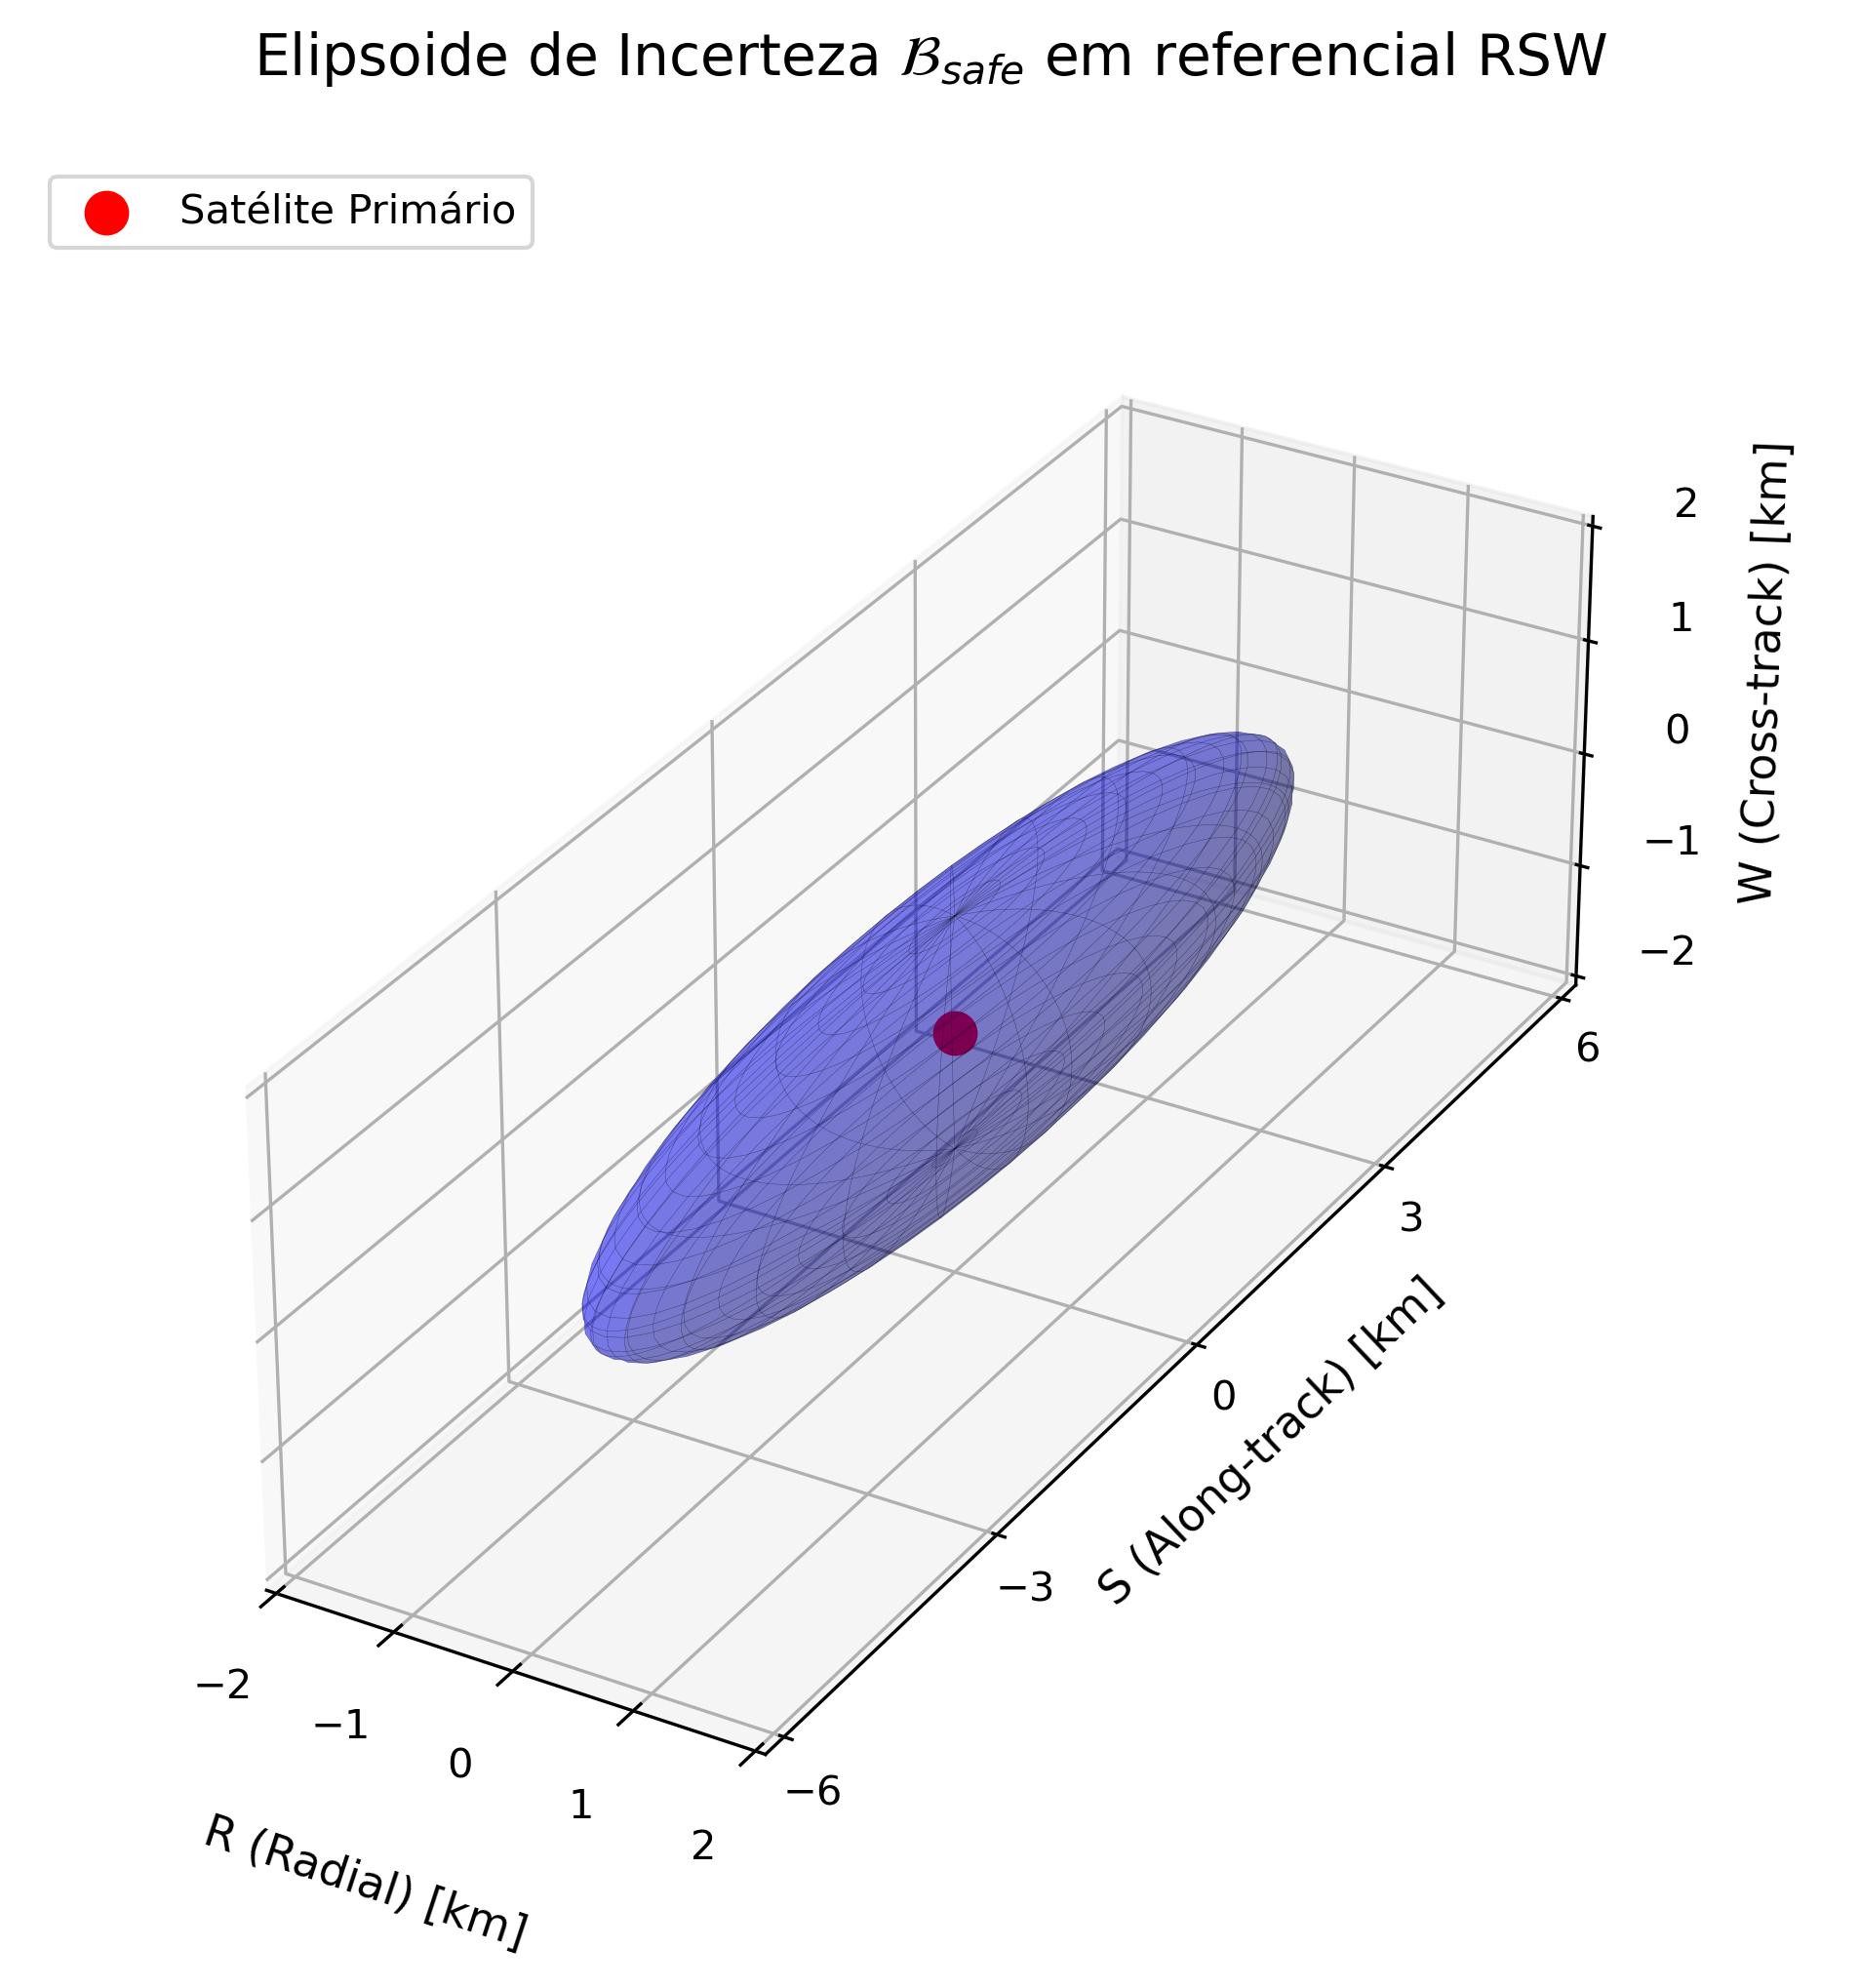
\includegraphics[width=0.85\textwidth]{docs/figuras/ellipsoid_3d.png}
    \caption{Arquitetura Geométrica tridimensional explícita do Limiar Determinístico em \textit{Concern List} desenhada sobre as margens reais das bordas de segurança contidas no escopo da base $\mathcal{B}_{safe}$ (1x5x1 km).}
    \label{fig:ellipsoid_3d}
\end{figure}

